\chapter{Neural Networks}

% Pridat uvodni povidani k sitim, proc, a co se deje v nasledujici kapitole
% ---------------------------------------------------------------------------

% Perceptron

A perceptron unit is able to find a linear boundary between two separable classes. In \emph{n}-dimensional space we talk about a separating hyperplane. The following equation \begin{equation} \bm{w}^\top \bm{x}+ w_{n+1} = 0\end{equation} is a vector form of the hyperplane equation, where $\bm{w}$ is a weight, \emph{n}-dimensional column vector, $\bm{x}$ is also \emph{n}-dimensional vector and it contains the coordinates of a point, which is being classified, $w_{n+1}$ is a bias. We can simplify the notation by creating a \emph{n+1}-dimensional vectors: $\bm{x} = [x_1, \dots, x_n, 1]^\top$ and $\bm{w} = [w_1, \dots, w_n, w_{n+1}]^\top$.
We want to find a weight coefficients that satisfies the following property:
\begin{equation}
\bm{w}^\top \bm{x} > 0 \qquad \bm{x} \in {class_1}\end{equation}
\begin{equation}
\bm{w}^\top \bm{x} < 0 \qquad \bm{x} \in {class_2}
\end{equation}
Then the perceptron learning algortihm can be described as follows:

For any $\bm{x}(k)$, at step $k$:
\begin{enumerate}
    \item If $\bm{x}( k ) \in class_1$ and $\bm{w}^\top \bm{x} \leq 0$ , let    
    \begin{equation}\bm{w} ( k + 1 ) = \bm{w} ( k ) + \alpha  \bm{x }( k )\end{equation}
    \item If $\bm{x}( k ) \in class_2$ and $\bm{w}^\top \bm{x} \geq 0$ , let   
    \begin{equation}\bm{w} ( k + 1 ) = \bm{w} ( k ) - \alpha  \bm{x }( k )\end{equation}
    \item Otherwise, let 
    \begin{equation}\bm{w} ( k + 1 ) = \bm{w} ( k )\end{equation}
\end{enumerate}

where $\bm{w}(1)$ is arbitrary and $\alpha > 0$ is a constant called learning rate. Sum of the products, $\sum_{k=1}^{n}w_kx  + w_{n+1}$ is then passed through an activation function. In case of perceptron it is a threshold function returning either 1, when $\bm{x}$ belongs to $class_1$, or -1 when it belongs to the second class $class_2$. In Figure \ref*{img:percneuron}.a.
is shown a model of a perceptron.\cite{raisi2020text}

% obrazky perceptronu a neuronu vedel sebe, l jsou vrstvy
\begin{figure}[hbtp]
    \centering
    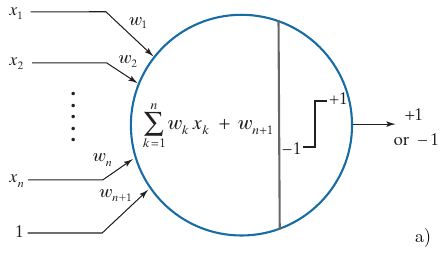
\includegraphics[scale=0.41]{obrazky/perceptron.png}
    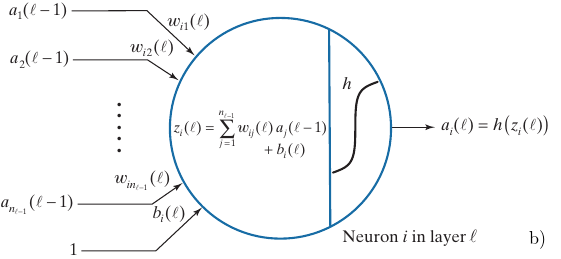
\includegraphics[scale=0.41]{obrazky/artneuron.png}

    \caption{Model of a perceptron unit (a), model of an artificial neuron (b) with used operations. The letter $h$ denotes an activation function, $l$ denotes a particular layer in a multilayer network. The element on the right is sometimes called a sigmoid neuron.\cite{DIP}}
    \label{img:percneuron}
\end{figure}

Linearly separable data are rather rare in real life problems. One possibilities is to use more perceptron units, however, the solution comes with neural networks and computing elements called artificial neurons. These elements are similar to perceptrons as they perform the same computations, but have a different attitude to processing the results. Schematics of a perceptron unit and an artificial neuron can be comapred in figure \ref*{img:percneuron}.
The perceptron activation function is very insensitive to small signals which can lead to false results. If the activation function is changed from a hard threshold to smooth function, results are then handled more carefully. There are few commonly used smooth activation functions, such as sigmoid, hyperbolic tangent or ReLu (rectifier linear unit) function. In Figure \ref*{img:actfunc} are the equations and shapes of the mentioned functions.\cite{DIP}

\begin{figure}[hbtp]
    \centering
    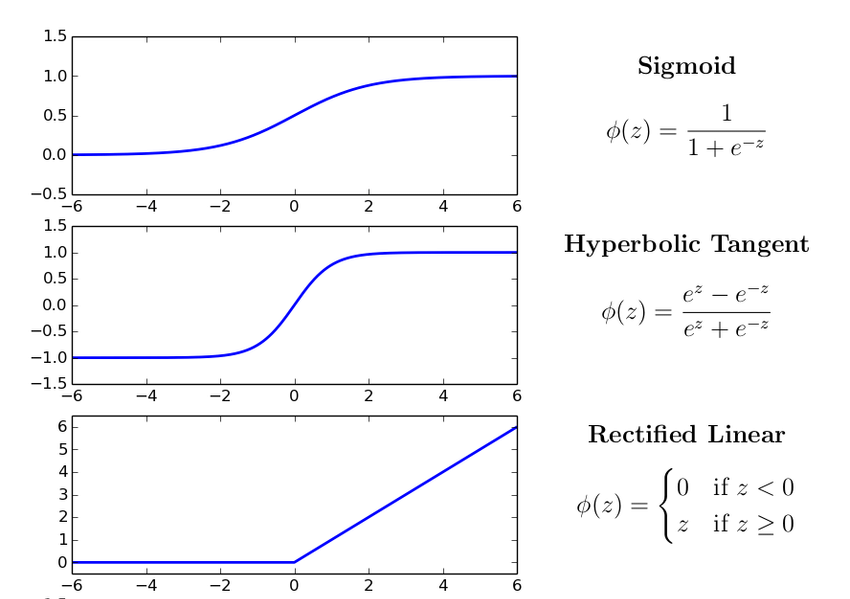
\includegraphics[scale=0.4]{obrazky/Common-neural-network-activation-functions.png}

    \caption{Commonly used activation functions in neural networks.\cite[altered]{activation}}
    \label{img:actfunc}
\end{figure} 
A generic neural network is depicted in Figure \ref*{img:fullyNN}.  By layer we understand a group of neurons, usually symbolized in a column. First layer contains the input vector $\bm{x}$, then every other layer contains the activation values of neurons in this layer. The conntecting lines between each two neurons signifies a fully connected neural network, where  output of every neuron from one layer is used as input for neurons in the following layer. Values of initial layer are known and also are the last output values, all neurons (and layers) between first and last layer are therefore called hidden. When there are more then one hidden layer we talk about deep neural network. Usually the number of output neurons is equal to the number of observed classes. For the rest of this chapter we will assume that there are no loops in the network.\cite{DIP}

\begin{figure}[hbtp]
    \centering
    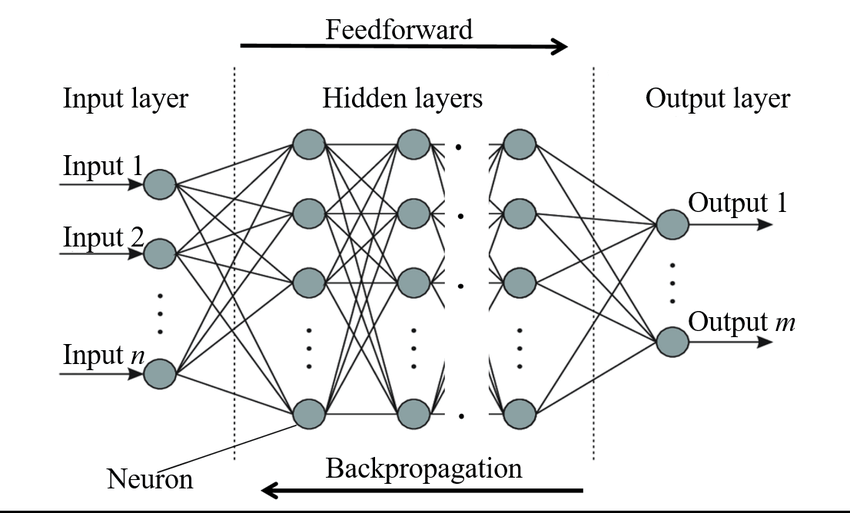
\includegraphics[scale=0.4]{obrazky/fullyNN.png}

    \caption{Fully connected neural network with processes.\cite{nn1}}
    \label{img:fullyNN}
\end{figure}

A forward pass through neural network maps the values of vector $\bm{x}$ (the input layer)  to the output layer, thus to determine the class of the vector $\bm{x}$. Steps of a forward pass can be written in matrix notation. This aproach is good for computing simultaneously with multiple input vectors and all neurons in one layer. The forward pass can be described in three steps:

\begin{enumerate}
    \item Input \begin{equation}\bm{A}(1)=\bm{X}\end{equation}
    \item Feedforward step 
    \begin{equation}\mbox{For } l = 2, \dots, L \qquad \bm{Z}(l) = \bm{W}(l)\bm{A}(l-1)+\bm{B}(l) \mbox{, } \bm{A}(l)=h(\bm{Z}(l))\end{equation}
    \item Output \begin{equation}\bm{A}(L)=h(\bm{Z}(L))\end{equation}
\end{enumerate}

Matrix $\bm{W}(l)$ contains all weight vectors of all nodes in one layer $l$, $\bm{X}$ contains input vectors, $\bm{A}(l)$ contains output values from layer $l$, $\bm{B}$ is the matrix of biases, $\bm{Z}(l)$ contains the net inputs to neurons in layer $l$, $h$ is an activation function. This process of predicting works when we know the right values of weights and biases. These can be obtained by training a neural network via backpropagation.\cite{DIP}

During training of neural network we work with data where it is known for each sample to which class it belongs. This means that we know the values of all otuput neurons in the net. However, we do not know the values of outputs of hidden neurons. A process called backpropagation is used to obtain information about hidden neurons. It can be devided into four steps. These steps are repeated until the value of cost function is reduced to a desired level. One repetition is called an epoch, thus the number of iterations is the number of epochs used for training the network.\cite{DIP}

\begin{enumerate}
    \item Input of data from training set.
    \begin{equation}\bm{A}(1)=\bm{X}\end{equation}
    \item A forward pass to classify the data into class and determine the error of misidentified classes (sometimes this error function is called cost function) based on ground thruth from the training data.
    \begin{align}
        \begin{split}
            \mbox{For } l = 2, \dots, L \qquad & \bm{Z}(l) = \bm{W}(l)\bm{A}(l-1)+\bm{B}(l) \mbox{, }  \\
            & \bm{A}(l)=h(\bm{Z}(l)) \mbox{, }  \\
            & \bm{D}(L)=(\bm{A}(L)-\bm{R}) \odot h'(\bm{Z}(L))
        \end{split}
    \end{align}

    \item A backward pass that sends the output error back through the network, where changes to update neuron paramters are computed.
    \begin{equation}
        \mbox{For } l = L - 1 , L - 2 , \dots , 2 \qquad \bm{D}(l) = ( \bm{W}^\top ( l + 1 ) \bm{D} (l + 1 ) \odot h' ( \bm{Z} (l) )
    \end{equation}
    \item An update of weights and biases of neurons.
    \begin{align}
        \begin{split}
            \mbox{For } l = 2, \dots, L \qquad & \bm{W}(l) = \bm{W}(l) - \alpha \bm{D}(l)\bm{A}^top(l-1) \mbox{, }  \\
            & \bm{b}(l)= \bm{b}(l) - \alpha  \sum_{k=1} ^{n_p}  {\delta}_k(l) \mbox{, }   \\
            & \bm{D}(L)=(\bm{A}(L)-\bm{R}) \odot h'(\bm{Z}(L)) \mbox{, }  \\
            & \bm{B}(l) \mbox{ consist of horizontally stacked vectors } \bm{b}(l) \\ 
            & \mbox{for } n_p \mbox{ times,} \\
            & \bm{\delta}_k(l) \mbox{ are the columns of matrix } \bm{D}(l) \mbox{,}
        \end{split}
    \end{align}
\end{enumerate}
where $\bm{W}(l)$ is the matrix of weights of all nodes in one layer $l$ for the inputs from $\bm{X}$, which contains multiple input vectors, $\bm{A}(l)$ contains output activation values from layer $l$, $\bm{B}$ are the biases, $\bm{Z}(l)$ contains the net inputs to neurons in layer $l$, $\bm{\delta}(l)$ tells us the rate of error change with respect to a change in the net input to any neuron in the network $\delta_k(l) = $, $\alpha$ is the  learning rate used in training, $h$ is an activation function.  
$\bm{W}(1)$ and  $\bm{B}(1)$ are set as random small numbers when initializing the process.\cite{DIP}

The error function for all output neurons for a single input $\bm{x}$ is defined as
\begin{equation} E = \sum_{j=1} ^{n_L} E_j = \frac{1}{2}\sum_{j=1} ^{n_L} (r_j-a_j(L)) = \frac{1}{2} ||\bm{r} - \bm{a}(L)||^2 \end{equation}

where $\bm{r}$ is a desired response for a given input $\bm{x}$, $\bm{a}(L)$ is the output of last layer in the network, in the last term is used the notation of the Euclidan vector norm. The error for all input vectors\footnote{a total  network output error} is equal to the sum of the individual errors.\cite{DIP}

\section{Convolutional Neural Networks}

The procedures described in the previous part dealt only with the case where the input data are in the form of a vector. In optical character recognition we work with image data that are not primarily represented as vector but as a matrix of pixel values. The matrix can be linearized from 2D to 1D when indeces are mapped gradually. However,  this approach does not consider spatial relationships that may be present among specific pixels. For examples edge or color similarities which are significant in text detection. Convolutional neural network (CNN) accepts 2D matrix as input and extracts features from the given image, these features are then fed to a classic fully connected neural network. A diagram describing  a simple CNN is in Figure \ref*{img:CNN}. We will discuss individual steps visible in this figure below.\cite{DIP}

\begin{figure}[hbtp]
    \centering
    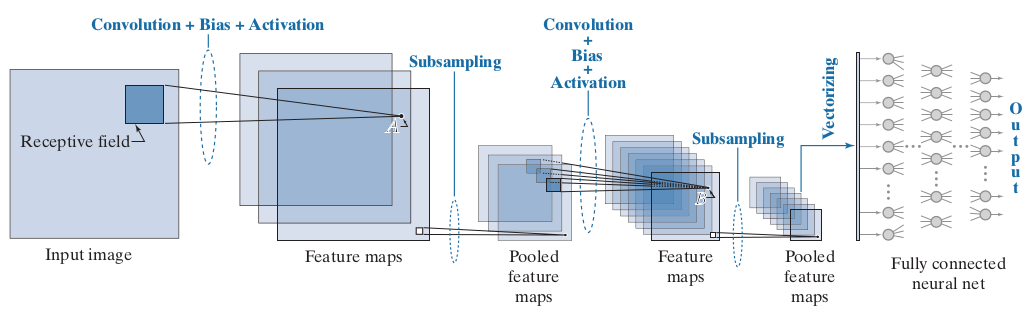
\includegraphics[scale=0.4]{obrazky/CNN.png}

    \caption{A simple CNN with LeNet architecture.\cite[altered]{DIP}}
    \label{img:CNN}
\end{figure}

First, a region of of pixels of the input image, a receptive field,  is selected. This field is moved over the image with a certain step. At each position a convolution is performed and values are stored in a 2D matrix. The size of the step determines the size of the resulting matrix (for example step of size two reduces the resolution of the image by one half). A mathematical definition of convolution operation is written in Definition \ref*{math:def:conv}. To each value obtained by convolution a bias is added and then is passed through an activation function. The new matrix thus obtained is called feature map. A single feature map is generated with same weights in convolution kernel and same bias, because this way a same feature is detected through the image. For another feature map different weight and bias is used. A group of feature maps in a CNN are called a convolutional layer. After the convolution step pooling is performed (sometimes called subsampling).\cite{DIP}

\begin{definition}
    Let $f(x,y)$ be in image and $w$ a kernel of size $m \times n$. Convolution with kernel $w$ is denoted as 
    $(w\star f)$     and defined as
    \begin{equation}
        (w\star f)(x,y) = \sum_{u=-k} ^{k} \sum_{v=-l} ^{l} w(u,v) f(x-u, y-v).
    \end{equation}
    \label{math:def:conv}
\end{definition}

Pooling is responsible for reduction of output dimension and causes a translational invariance. It is done by dividing a feature map into $2 \times 2 $ adjacent (non-overlapping) regions, the four values in this region are replaced by only one value. Common pooling methods are: average pooling, the values in region are replaced by the average of the values; max pooling, the values are replaced by the maximal value from the region; $L_2$ pooling, the final value is obtained by computing the Euclidan norm of the four values. We obtain one matrix for each feature map from the convolution step. The bunch of matrices from the pooling step is called a pooling layer. The result of the last pooling layer is vectorized and sent to the fully connected neural network. The training procedure of the CNN is analogical to the training of a fully connected neural network. However, convolution is used instead of matrix multiplication and the output from fully connected network has to be converted into 2D matrix.\cite{DIP}

\section{Recurrent Neural Networks}
\label{sec:RNN}

Recurrent neural networks (RNN) same as feedforward networks has an input, hidden and output layer. Unlike the classic networks RNNs share parameters (weights and biases) across each layer of the network and they remember results of computations. This approach is very useful in contextual tasks such as language problems (speech and written text recognition) where the position of a word in a sentence and surrounding words can help predict text.

During training of RNN errors from output to input layer are calculated but unlike in standard backpropagation the errors are summed up because of the shared parameters. This process makes RNNs prone to two problems called exploding and vanishing gradients. The former one happens when gradients are large and by summing they enlarge too much to be represented as undefined (NaN) value, which leads to instability of the model. The latter refers to the case when gradients are contrarily too small, they continue to decrease and the weights become insignificant.\cite{rnn}

\subsection*{Long short-term memory}
\label{sec:LSTM}

Long short-term memory (LSTM) is a type of RNN. It contains so-called memory blocks, which are memory blocks (cells) located in the hidden recurrent layer. Each memory block contains three gates -- input, output and forget gate. The input one controls the flow of information in to the cell. The output gate controls what information is to be passed to the rest of the network. The forget gate was added later and it manages the amount of information stored in cell before new information is received. Generally the cell input and cell output activation functions is $\tanh$ and the network activation function is softmax. A scheme of LSTM is in Figure \ref*{img:LSTM}.\cite{lstm}

LSTM network has some variations. It is possible to stack LSTM layers on top of each other between the input and output layer and create a deep LSTM. Another type is a bidirectional LSTM (BLSTM) which differs from normal LSTM that it remembers not only information from the past but also from the future (e. g. when the model wants to predict a word in a sentence, it knows all the words behind the currently predicted word and also all the following words). It enables better usage of contextual information which is crucial in language processing.\cite{lstm,baueldungLSTM}

\begin{figure}[hbtp]
    \centering
    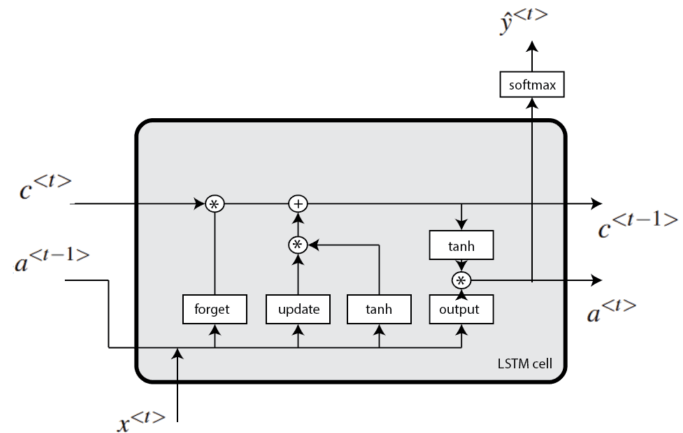
\includegraphics[scale=0.4]{obrazky/lstm.png}

    \caption{Scheme of a LSTM recurrent neural network.\cite{baueldungLSTM}}
    \label{img:LSTM}
\end{figure}


\section{Convolutional Recurrent Neural Networks}
\label{sec:CRNN}

Convolutional recurrent neural network is a type of a neural network designed for the purposes of image object recognition. It was introduced by Shi and al. \cite{crnn} in the year 2015. It combines the advantages of a deep CNN and RNN. It reads directly features from image data without prior feature extraction or image preprocessing such as binarization as CNN does. It produces a sequence of labels as RNN. Further it has no restriction on the length of an object (texts are rather long and flat), it can learn from words so there is no need to segment text to individual characters. CRNN also has a smaller amount of parameters than a deep CNN thus it requires less storage space.\cite{crnn}

\begin{figure}[hbtp]
    \centering
    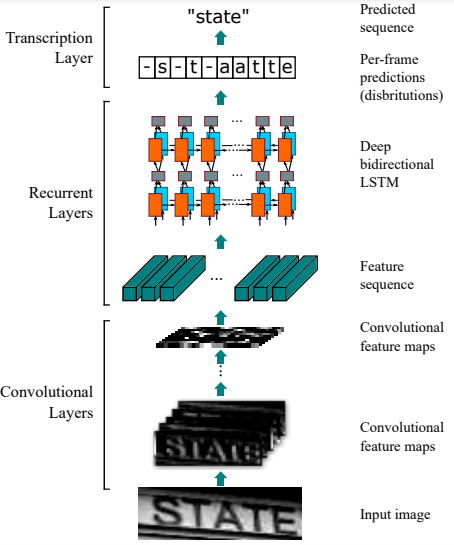
\includegraphics[scale=0.46]{obrazky/crnn.png}

    \caption{An architecture of CRNN for recognizing objects in images.\cite{crnn}}
    \label{img:CRNN}
\end{figure}

First CNN with max pooling extracts features directly from the image input. The convolutional layers are followed by recurrent ones, which take the frame output of CNN and predict labels for each frame, then a transcription layer translates the segmented labels into a continuous text. This architecture is visible in Figure \ref*{img:CRNN}.

The images, that are to be recognized, are scaled to the same height and then feature map is obtained by CNN. Feature
vectors are extracted from each column of the feature map, so a vector covers a rectangle area of the input image. This are is called a receptive field. CRNN uses then a deep bidirectional LSTM network to predict labels. During transcription the model picks the label of a frame which has the highest probability. This can be made either with a help of a lexicon or without it.\cite{crnn}









